\documentclass[11pt,a4paper]{ctexart}
\usepackage[margin=2cm]{geometry}
\usepackage{booktabs,longtable,tabularx,array,graphicx,xcolor,xurl}
\usepackage[colorlinks,urlcolor=blue,linkcolor=blue]{hyperref}
\setlength{\parindent}{0pt}\setlength{\parskip}{5pt}
\newcolumntype{L}[1]{>{\raggedright\arraybackslash}p{#1}}
\title{Demo 与图片制作清单\\\large 全流程数据、132维特征与多轮RSI版本}
\author{2026年11月12日 · 中文CVPR技术报告配套}\date{}
\begin{document}\maketitle
\textbf{已经有可用的demo基础。}本地找到六段交互图视频，最新为\path{demo_v6.mp4}；本稿已按这些实际资产重新盘点。项目方确认最终全量结果约0.93，素材应围绕最终RSI冠军组织。主要缺口是最新冠军与数据绑定、逐轮RSI记录、最终分层指标及正式导出的可读性。

\section{已找到的实际素材}
路径相对于\path{/home/nvidia/algotithm/demo/}。下列规格来自本地ffprobe，六段均为1500$\times$500像素；播放帧率不等于原视频采样率或模型推理速度。
\begin{longtable}{L{4.9cm}L{2.7cm}L{6.7cm}}
\toprule 文件 & 实际规格 & 用途\\\midrule\endhead
\path{b857b2a8_demo.mp4} & 6秒，24帧，4fps & 早期三栏交互关系演示，作为版本对照留档。\\
\path{b857b2a8_demo_v2.mp4} & 6秒，24帧，4fps & 放大版，可对照可读性迭代。\\
\path{e923ec44_demo.mp4} & 2秒，8帧，4fps & 补充场景短片，需核对划分和模型来源。\\
\path{demo_pose_v4.mp4} & 10.75秒，43帧，4fps & 手／物位姿与关系图版本，需说明缺失几何的回退。\\
\path{demo_v5.mp4} & 8秒，24帧，3fps & 连续采样的演示迭代版本。\\
\path{demo_v6.mp4} & 8秒，24帧，3fps & 最新本地三栏：RGB、复核关系、LSTM预测；适合作为主片基础。\\\bottomrule
\end{longtable}
规格和SHA保存在\path{evidence/current_demo_inventory.json}。原始\path{preview_v6.png}已作为报告真实预览帧。
\begin{center}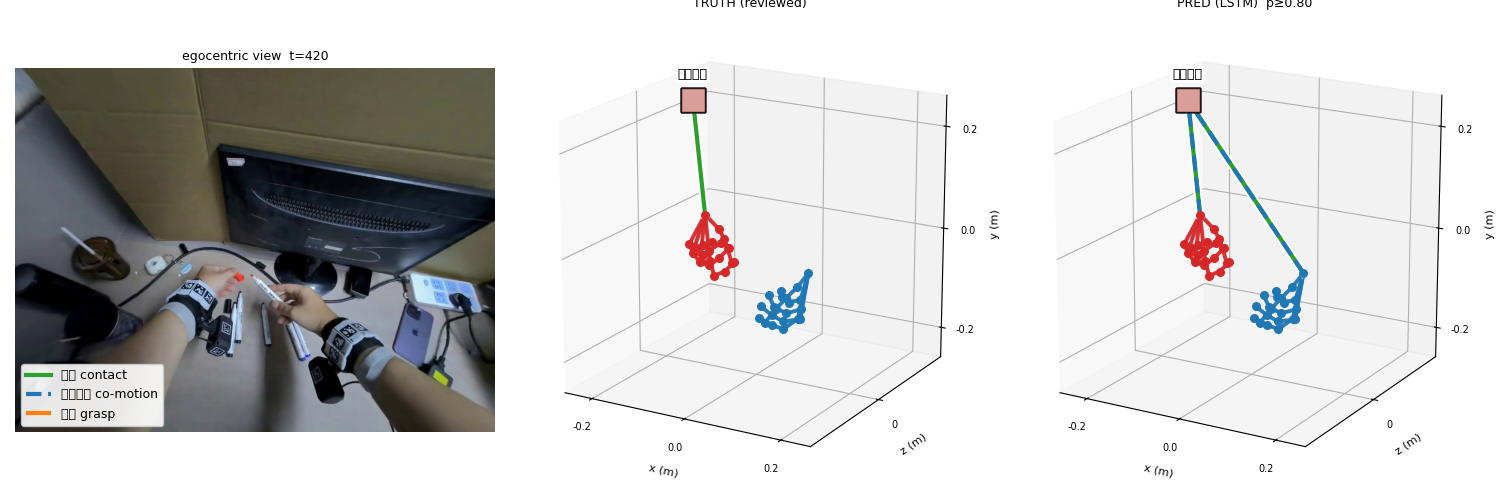
\includegraphics[width=\linewidth]{figures/demo_v6_actual.png}\end{center}
\textbf{v6画面需处理：}部分中文仍显示方框，重渲染需指定CJK字体；预测栏写明LSTM与显示阈值0.80；中栏“TRUTH (reviewed)”应准确标注复核来源；手部骨架和物体位姿是观测，不是未来姿态预测。缺失几何应明确显示缺失，不使用无说明的假定深度。

\section{优先补齐的文件}
“待同步”仅表示本次未直接读取最新服务器文件，不表示项目尚未完成相关工作。
\begin{longtable}{L{.9cm}L{3.3cm}L{10.1cm}}
\toprule 级别 & 素材 & 内容与验收\\\midrule\endhead
P0 & 最终0.93的结果绑定 & 最终run、完整指标键／精确值、test benchmark、config、checkpoint SHA、评估器版本、阈值、随机种子、数据索引与准入文件。先回收记录，无需先重跑训练。\\
P0 & 全部RSI系列账本 & rsi\_v5、rsi\_auto、rsi\_final的history、REPORT、genome、候选score与选择记录；区分尝试、成功评分、失败、晋升。不同数据版本分别作图。\\
P0 & 最终数据统计 & 冠军绑定索引的train/val/test采集与窗口数、有效监督采集数、四层正负／未知、实体与类型支持数。300段资源池和289段处理范围不替代有效训练规模。\\
P0 & 冠军逐窗口输出 & sequence ID、历史起止、anchor／target原生帧与时间戳、实体映射、类型词表、概率、评估／显示阈值、标签与mask、checkpoint SHA。\\
P0 & 原片与渲染脚本 & demo对应原始连续视频、采样帧清单、手／物观测、位姿来源与有效性、视觉名到几何名映射、渲染配置及字体。已有短片可剪辑，修字和绑定冠军仍需原数据。\\
P1 & 同版本对照与分层指标 & 初始配置、RSI冠军、三骨干使用相同数据／特征；每层P/R/F1和支持数。全正参照按最终已知标签重算，不复用旧子集数字。\\
P1 & 成功、失败、未知案例 & 按固定规则选择最终测试窗口；至少一个误报／漏报和一个遮挡未知。保存候选列表与选择原因。\\
P2 & 端到端实测录屏 & 仅在需要强调在线／实时能力时补录，说明采样率、感知／推理延迟、硬件与离线候选条件。\\\bottomrule
\end{longtable}

\section{论文配图安排}
\begin{longtable}{L{.8cm}L{3.3cm}L{7.2cm}L{2.7cm}}
\toprule 图号 & 内容 & 文件／制作要求 & 状态\\\midrule\endhead
F1 & 120／132维系统结构 & figures/architecture.pdf；特征、空间注意力、时间骨干、有向图头与监督。 & 已生成矢量图\\
F2 & RSI机制 & figures/rsi\_loop.pdf；受约束变异、验证选择、失败留档与晋升。 & 已生成矢量图\\
F3 & 同版本骨干结果 & figures/expanded\_results.pdf；目前为10月26日历史输出；正式主表待换入最终同版本结果。 & 阶段结果可用\\
F4 & 历史版本概览 & figures/version\_history.pdf；各组对应不同测试集，只说明演进。 & 历史图可用\\
F5 & 真实三栏demo & figures/demo\_v6\_actual.png；正式导出修复字体并核对冠军。 & 已有真实预览\\
F6 & RSI逐轮／晋升曲线 & 横轴为唯一候选或累计训练预算，纵轴同版本val micro-F1；失败单列，标注晋升。 & 待完整账本\\
F7 & 最终数据与分层指标 & 划分、正负未知、四层P/R/F1与支持数；注明统计分母。 & 待最终索引／评估\\
F8 & 提前预测和错误案例 & 2行$\times$4格：历史、截止、预测、目标揭示；成功与失败对照，未知单列。 & 待冠军逐窗输出\\\bottomrule
\end{longtable}
结构与统计图保留PDF矢量；真实帧保存原分辨率PNG。最终栏宽下中文须可读，实体名称和颜色统一；位姿缺失与标签未知分开表达。

\section{主视频分镜：110秒}
以下为剪辑计划，不是已录视频时间戳。复用现有短片，补足最终模型绑定后正式导出。
\begin{longtable}{L{1.5cm}L{3.6cm}L{9.2cm}}
\toprule 时间 & 画面 & 旁白／输入\\\midrule\endhead
00--08 s & 真实操作与任务 & 从过去手物状态预测约一秒后交互；若用离线位姿候选，在输入条件角标说明。\\
08--22 s & 数据与系统 & 最终有效采集／窗口统计；依次展示120／132维输入、空间编码、时间骨干与交互图。\\
22--38 s & 多轮RSI & 真实候选评分与晋升，不同版本分面；展示冠军配置和最终约0.93的精确指标。\\
38--66 s & 连续成功例 & 历史与冻结预测先显示，推进原生时间轴后揭示目标复核标签。字幕给主体、客体、类型、概率。\\
66--84 s & 同窗口对照 & 初始配置与冠军使用同一窗口、特征和阈值；三骨干对照也必须使用最终同版输出。\\
84--102 s & 失败与未知 & 一个误报／漏报和一个遮挡未知；模型概率与有效标签对照，未知不计作正确或错误。\\
102--110 s & 最终结果卡 & 指标名称、最终测试规模、评估阈值及输入条件；封面突出RSI优化后的意图预测。\\\bottomrule
\end{longtable}
建议1920$\times$1080 H.264，保持原图比例与原生时间轴，低采样回放标明倍率。0.80显示阈值可减少边拥挤，但指标卡必须使用benchmark实际阈值；目标到来前不展示未来标签。

\section{交付验收与同步入口}
\begin{enumerate}
\item 用demo\_manifest.json绑定模型、数据、词表、评估器、逐窗输出与SHA；不能凭文件名final判定冠军。
\item 修复中文，核对实体和交互类型；准确说明复核来源、观测位姿与预测边。保留缺失和未知状态。
\item 完整解码，抽查首尾、遮挡与时间戳；确认观察截止前没有目标标签，保留失败例。
\item 导出主片、无字幕片、中文字幕SRT、关键帧、逐窗JSONL、封面和来源表；数值与正文一致。
\end{enumerate}
优先读取\path{/root/gpufree-data/runs/}下的rsi\_final、rsi\_auto、graph\_v5\_auto，并回收rsi\_v5补全历史；数据目录由run配置确定。\path{scripts/collect_remote_evidence.py}可只读打包这些系列的小型记录和checkpoint哈希，也可显式指定数据根收集索引／发布摘要；本次未在服务器执行。

旧五段MP4备份的LFS指针问题不影响已经存在的六个可解码demo；正式重渲染仍需对应原片。技术报告、素材清单与现有演示视频均为本地交付，未公开发布。
\end{document}
